\documentclass[tikz,border=10pt]{standalone}
\usepackage{tikz}
\usepackage{tikz-3dplot}
\usetikzlibrary{shapes.geometric, arrows.meta, fit, backgrounds, angles, quotes}

\begin{document}
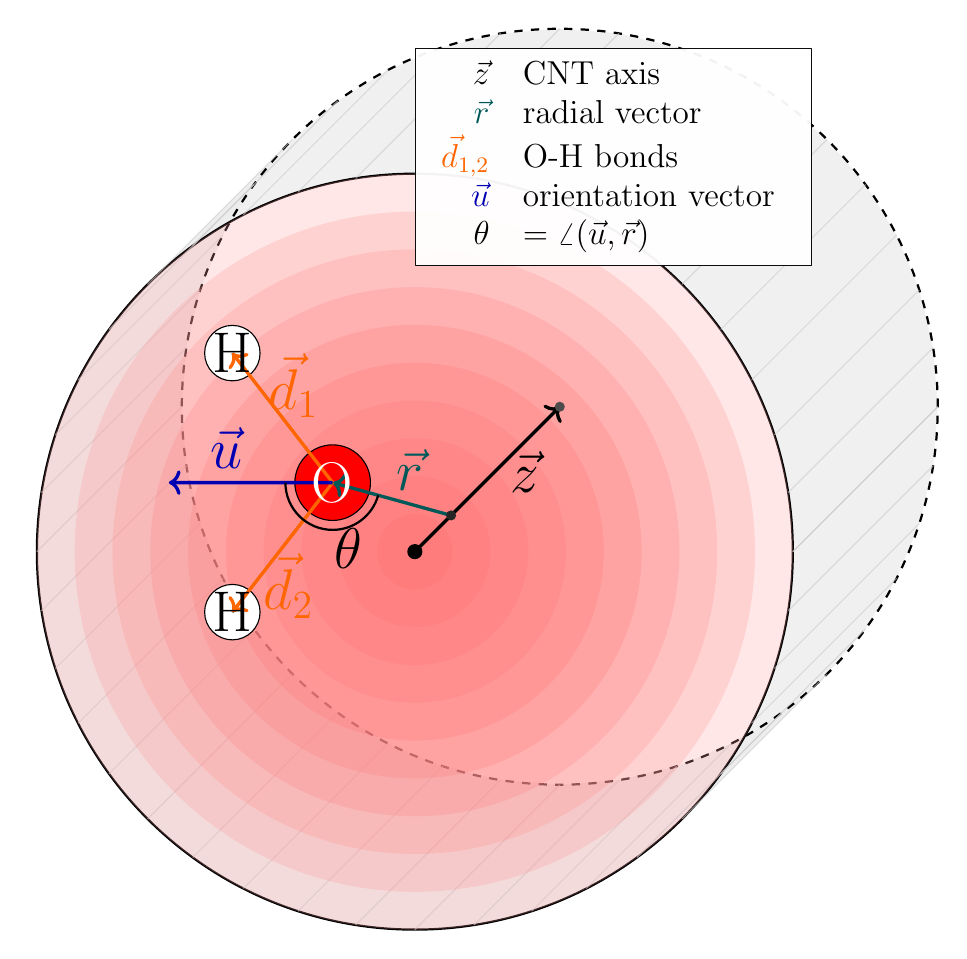
\begin{tikzpicture}[scale=3.2, line join=round]

  \def\R{1.5}
  \def\H{3}
  \def\Steps{10}
  \def\bondlength{0.65}
  \def\angleHOH{127.75}

  % Colors and styles
  \tikzset{
    vect-CNT/.style={->, very thick, black},
    vect-perp/.style={->, very thick, teal!70!black},
    vect-OH/.style={->, very thick, orange!80!red},
    vect-mol/.style={->, very thick, blue!70!black},
  }

  % Cylinder
  \coordinate (O) at (0,0,0);
  \coordinate (A) at (2.5,2.5,5);

  % Make CNT slightly more transparent for better contrast
  \foreach \i in {0,...,39} {
    \pgfmathsetmacro{\angleA}{\i*360/40}
    \pgfmathsetmacro{\angleB}{(\i+1)*360/40}
    \path (O) ++(\angleA:\R) coordinate (PF1);
    \path (O) ++(\angleB:\R) coordinate (PF2);
    \path (A) ++(\angleA:\R) coordinate (PB1);
    \path (A) ++(\angleB:\R) coordinate (PB2);
    \fill[gray!15, opacity=0.8] (PF1) -- (PF2) -- (PB2) -- (PB1) -- cycle;
  }

  \tdplotdrawarc[thick,dashed] {(A)}{\R}{0}{360}{}{}
  \tdplotdrawarc[thick] {(O)}{\R}{0}{360}{}{}

  % Improve grid lines
  \foreach \i in {0,...,40} {
    \pgfmathsetmacro{\angle}{\i*360/40}
    \path (O) ++(\angle:\R) coordinate (P);
    \path (A) ++(\angle:\R) coordinate (Q);
    \draw[thin,gray!40, opacity=0.6] (P) -- (Q);
  }

  \foreach \i in {1,...,\Steps} {
    \pgfmathsetmacro{\rstep}{\i*\R/\Steps}
    \pgfmathsetmacro{\shade}{100 - (\i-1)*70/\Steps}
    \tdplotdrawarc[fill=red!\shade, draw=none, opacity=0.25]
      {(O)}{\rstep}{0}{360}{}{}
  }

  \draw[vect-CNT] (O) -- (A) node[pos=0.55, right=2pt] {\huge $\vec{z}$};

  % Water molecule
  \coordinate (Oxy) at ($(O)!0.65!(A) + (-0.7,-0.1,0)$);
  \path (Oxy) ++(\angleHOH:\bondlength) coordinate (H1);
  \path (Oxy) ++(-\angleHOH:\bondlength) coordinate (H2);
  \path (Oxy) ++(180:\bondlength) coordinate (mid);

  \def\rO{0.15}
  \def\rH{0.11}

  \fill[red] (Oxy) circle[radius=\rO];
  \fill[white] (H1) circle[radius=\rH];
  \fill[white] (H2) circle[radius=\rH];
  \draw[black,thin] (H1) circle[radius=\rH];
  \draw[black,thin] (H2) circle[radius=\rH];
  \draw[black,thin] (Oxy) circle[radius=\rO];

  % Bond lines (edge to edge)
  \path let \p1 = (Oxy), \p2 = (H1) in
    coordinate (H1in) at ($ (Oxy)!{\rO/veclen(\x2-\x1,\y2-\y1)}! (H1) $);
  \path let \p1 = (H1), \p2 = (Oxy) in
    coordinate (H1out) at ($ (H1)!{\rH/veclen(\x2-\x1,\y2-\y1)}! (Oxy) $);
  \draw[thick] (H1out) -- (H1in);

  \path let \p1 = (Oxy), \p2 = (H2) in
    coordinate (H2in) at ($ (Oxy)!{\rO/veclen(\x2-\x1,\y2-\y1)}! (H2) $);
  \path let \p1 = (H2), \p2 = (Oxy) in
    coordinate (H2out) at ($ (H2)!{\rH/veclen(\x2-\x1,\y2-\y1)}! (Oxy) $);
  \draw[thick] (H2out) -- (H2in);

  % Vectors
  \draw[vect-perp] ($(O)!0.25!(A)$) -- (Oxy)
    node[pos=0.35, above=1pt] {\huge $\vec{r}$};

  \draw[vect-OH] (Oxy) -- (H1) node[pos=0.75, right=0pt] {\huge $\vec{d}_1$};
  \draw[vect-OH] (Oxy) -- (H2) node[pos=0.8, right=0pt] {\huge $\vec{d}_2$};

  \draw[vect-mol] (Oxy) -- (mid) node[pos=0.65, above=1pt] {\huge $\vec{u}$};

  % Angle θ
  \coordinate (Z) at ($(O)!0.25!(A)$);
  \coordinate (V) at (Oxy);
  \coordinate (M) at (mid);
  \draw pic[
    draw=black,
    thick,
    angle radius=6mm,
    angle eccentricity=1.4,
    right=0pt,
    "\huge $\theta$"
  ] {angle = M--V--Z};

  % Atom labels
  \node[font=\scriptsize, white] at (Oxy) {\huge O};
  \node[font=\scriptsize, black] at (H1) {\huge H};
  \node[font=\scriptsize, black] at (H2) {\huge H};

  % Legend (in English)
  \node[draw, align=left, fill=white, opacity=0.95, text opacity=1, anchor=north west, font=\large] at (0,2) {
    \begin{tabular}{rl}
      \textcolor{black}{$\vec{z}$} & CNT axis \\
      \textcolor{teal!70!black}{$\vec{r}$} & radial vector \\
      \textcolor{orange!80!red}{$\vec{d}_{1,2}$} & O-H bonds \\
      \textcolor{blue!70!black}{$\vec{u}$} &  orientation vector \\
      \textcolor{black}{$\theta$} & $= \angle(\vec{u}, \vec{r})$ \\
    \end{tabular}
  };

  \fill[black] (O) circle[radius=0.03];
  \fill[black!70] (A) circle[radius=0.02];
  \fill[black!85] ($(O)!0.25!(A)$) circle[radius=0.02];

\end{tikzpicture}
\end{document}
